
\section{Численные эксперименты}\label{sec:experiments}
    Для демонстрации работы предложенного метода было проведено два эксперимента. Первый эксперимент основан на сценарии классической задачи линейного программирования, а именно на задаче производства. Во втором эксперименте рассматривается задача конкурирующих потоков минимальной цены (Minimum Cost Concurrent Flow, MCCF). В этом эксперименте целевые функции имеют похожую структуру, но отличаются в параметрах, отвечающих за сценарий использования сети. Код экспериментов расположен по адресу \url{https://github.com/intsystems/NIR_LatypovIM}.
    
\subsection{Задача производства}\label{exp:simple}
Идея эксперимента основана на классической задаче линейного программирования, но расширяет её.  Пусть дана компания, деятельность которой можно разделить на периоды. Компания производит $k$ видов продукции на сумму $x \in \mbR^k$ и реализует ее по стоимостям $c \in \mbR^k$.  Для этого компании требуется $n$ типов ресурсов со стоимостями $b \in \mbR^n$, которые приобретаются по цене $c_b \in \mbR^n$ в начале периода. Некоторые ресурсы могут закончиться в течение этого периода, поэтому компания может докупать недостающие ресурсы $y$ во время периода по повышенной стоимости $c_a \in \mbR^n$: $c_a \ge c_b$ - покомпонентно.  Для производства $i$-го продукта компания использует $j$-ый ресурс в количестве $a_{ij}$. Обозначим затраты ресурсов как матрицу $A = \|a_{i,j}\|_{i,j = 1}\in \mbR^{n \times k}$. 

Для упрощения выкладок и описания эксперимента предполагаем, что компания докупает недостающие ресурсы ровно столько, сколько ей нужно. Это реализуется, если компания заказывает малые порции ресурсов в покупках внутри периода.

В рассматриваемой постановке $x$ -- случайная величина, распределение которой неизвестно. Семплируется она один раз в период, так что собрать и исследовать большую выборку нет возможности. С учетом всех затрат, доход компании за рассмотренный период дается следующим выражением:
\begin{align*}        
    f(b, x, c, c_b, c_a) = c^Tx - c_b^Tb - c^T_a y \\
    y = \max(0, Ax-b)
\end{align*}

Эти функции Липшицевы, например в норме  $L_1$ с константами  $$\max(\text{abs} (c_b), \text{abs}(c_a - c_b))$$.

Пусть компания проработала $m$ периодов и пронаблюдала величины $i \in \overline{1, m}: c_i, x_i, c_b^i, c_a^i$ для начальных объемов ресурсов $b_i$.  Необходимо найти стратегию приобретения ресурсов в начале периода, которая даст достаточно хороший доход в случае, если ситуация будет похожа на одну из предыдущих. Естественным ограничением здесь является ограничение по бюджету: $K = \{b: c_b^T b \leq B\}$. В эксперименте мы  варьируем бюджет и получаем результаты. 

\subsubsection{Производство: результаты}
Рассматриваем количество случаев $m=50$, количество видов ресурсов $n = 80$, количество видов продуктов $k = 30$. Варьируем бюджет $B$. Для поиска приближенного решения используем нормы $\|\cdot\|_1$, $\|\cdot\|_2$ c точными константами Липшица. Также рассматриваем $\|\cdot\|_2$ в которой все константы Липшица заменены на значение 100. Все результаты сравниваются с точным решением \ref{opt:T1}.

На рисунке \ref{fig:simple:results} отображено среднее качество решения для разных бюджетов $B$. Точка представляет собой среднее качество решения, полученного алгоритмом для разных функций. А именно рассматривается отношение значений функции в найденной точке к значениям функций в исходных точках. Рисуется их среднее значение и дисперсия. Эти значения отображены на оси $y$. По Оси $x$ отложены бюджеты, для которых проводились вычисления. Слева направо изображены результаты для разных норм:  $\|\cdot\|_1$; $\|\cdot\|_2$; $\|\cdot\|_1$ с неточными константами -- все $ \widetilde{L}_i =100$. График справа представляет собой точное решение. Результаты визуально не отличимы в силу простоты рассмотренной задачи.

Чтобы увидеть различия, рассмотрим график с относительными значениями качеств решений: рисунок \ref{fig:simple:relations}. Из графика с точным решением вычитаем остальные графики и делим разность на точное решение для нормализации. Значение по оси $y$ выше для более качественного решения. Видно, что алгоритмы на норме $\|\cdot\|_2$ работают одинаково и качество их решения отличается от точного не более чем на 1\%. Норма $\|\cdot\|_1$ получает результаты хуже -- качество решениия ухудшается до 2\%. Объясняется это тем, что алгоритм получает более разреженное решение, что чаще приводит к нехватке некоторых ресурсов. Для всех норм видим ухудшение качества решения при некотором значении бюджета. Это случается из-за того, что алгоритм начинает закупать ресурсы, которые являются лишними для рассмотренных сценариев. 

\begin{figure}
\centering
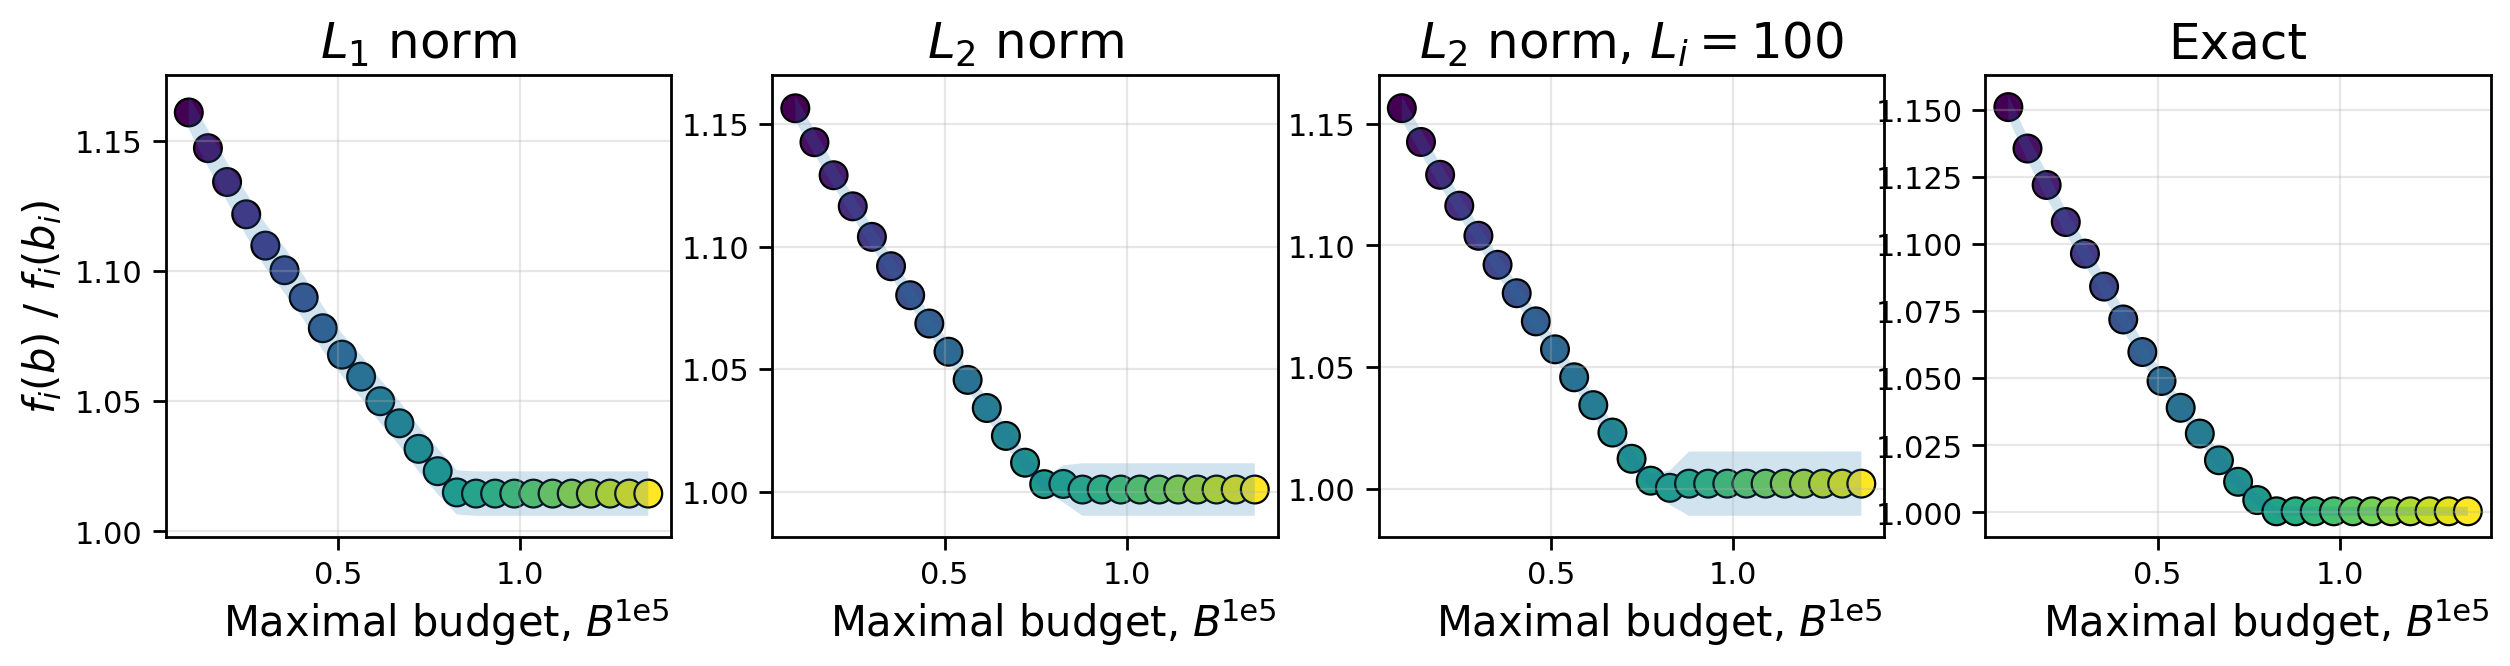
\includegraphics[width=\textwidth]{figures/simplest/relations.png}
            \caption{ Зависимость относительного прироста функции от бюджета для разных способов решения задачи производства.}
    \label{fig:simple:results}
\end{figure}
    
\begin{figure}
    \centering
    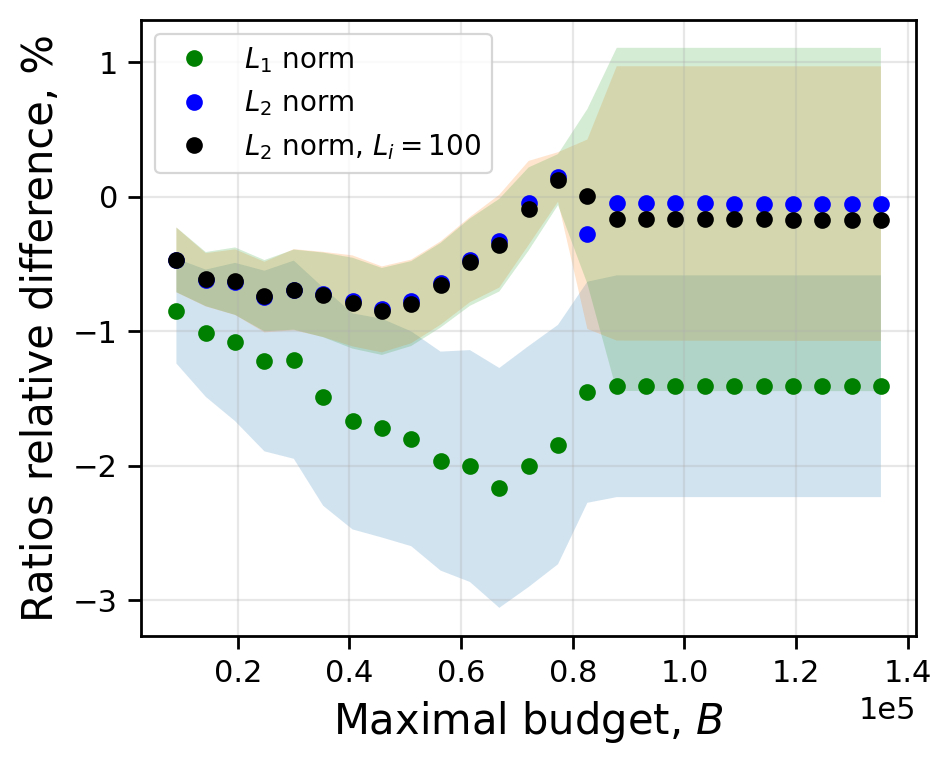
\includegraphics[width=0.5\textwidth]{figures/simplest/relative_difference.png}
    \caption{ Относительная разность качества приближенного решения с качеством точного решения для задачи производства.}
    \label{fig:simple:relations}
\end{figure}

\subsection{Конкурирующие потоки минимальной цены}\label{exp:concurrent}
Задача конкурирующих потоков минимальной цены (minimal cost multicommodity flow, MCF) ставится следующим образом: задан граф $\mathcal{G}(V, E)$, у которого $m$ вершин и $n$ ребер. У ребер $e \in E$  задана пропускная способность $b_e$ и стоимость единицы потока $c_e$ для этой пропускной способности.  Кроме графа заданы потоки, которые необходимо обеспечивать сетью: $(s_i, t_i, f_i)$. Эта тройка означает источник $s$, сток $t$ и требуемый объем потока $f$. Обозначим эти запросы через матрицу корреспонденций $D$: $\forall i: D_{s_i, t_i} = f_i$. Требуется найти потоки в графе  $F \in\mbR^{n\times m}$, которые обеспечат выполнение всех заказов при минимально возможной стоимости.

Задача переписывается в виде задачи линейного программирования \cite{bazaraa2011linear}. Для этого определяем матрицу смежности вершин и ребер $A \in \mbR^{m\times n}$. Каждый столбец содержит ровно два ненулевых значения. Столбец, соответствующий ребру $(i, j)$ содержит "$+1$" в строке  $i$, "$-1$" в строке $j$, и нули во всех других строках. Для каждой вершины вводится вектор поставок  $d_i \in \mbR^m$, он нужен для записи всех потоков, исходящих из этой вершины. При помощи матрицы корреспонденции $D$ компоненты $d_i$ расписываются в виде:
\begin{equation*}
d_{ij} = 
\begin{cases}
    \sum_{k \neq j} D_{ik} & i == j \\
    -d_{ij}
\end{cases}
\end{equation*}

Соединим эти вектор-столбцы в матрицу и обозначим её $D_A \in \mbR^{m\times m}$, эта матрицы используется для удобной записи задачи. 
Используя \cite{bazaraa2011linear}, мы записываем оптимизационную задачу следующим образом:

\begin{align*}
    \min_{F} c_e^T F \textbf{1} & \\
    \text{s.t.} & ~ F\textbf{1} \leq b \\
                & ~ AF = D_A\\
\end{align*}

в этой формулировке задача может не иметь выполнимой точки в силу ограничения с  $b$. Чтобы убрать ограничения по $b$ и сделать задачу проще добавим штраф $y$ к задаче:
\begin{align*}
    \min_{F} c^T F \textbf{1} + c_a^T y & \tag{$MCF$}\label{opt:MCF}\\
    \text{s.t.} & ~ F\textbf{1} \leq b + y\\
                & ~ AF = D_A\\
\end{align*}

Этот штраф интерпретируется как аренда дополнительной пропускной способности в сети. Обозначим $g(b, D) = \text{value}(MCF(b, D))$.

Теперь опишем сценарий использования метода. Есть некая компания, которая предоставляет услугу доставки посылок/сообщений в некой сети. Для работы ей необходимо арендовать полосу пропускания. Она может арендовать полосу пропускания в начале периода по цене $c_b$ и арендовать дополнительную полосу пропускания в течение периода по цене $c_a$. На практике это происходит поэтапно, поскольку она арендуется заранее на длительный срок. В каждый период времени существуют требования на поставки -- матрица корреспонденции $D_i$, потоки из которой необходимо выполнить. Эти матрицы задают сценарии использования сети.  Компании они не известны на момент начала периода. Пусть она в течение $m$ периодов работала с разными арендованными мощностями $b_i$ и пронаблюдала $D_i$. В конце периода она подводит итоги и наблюдает свои расходы внутри периода $f_i(b_i) =g(b_i, D_i)$. Эти функции удовлетворяют условиям Липшица. Необходимо при заданном бюджете закупить пропускную способность так, чтобы она обеспечила небольшие траты для разных ситуаций. Компании на данный момент известны только те $D_i$ которые она пронаблюдала. Тут и появляется необходимость решать задачу \ref{opt:T1}. Ограничения $K = \{b: c_b^T b \leq B\}$.

\subsubsection{Конкурирующие потоки минимальной цены:результаты}

 В эксперименте используем топологию "germany50" ~~ из датасета SNDLib \cite{orlowski2010sndlib}. Это сеть из 50 вершин и 176 ребер. В датасете совместно с самим графом приводится набор матриц корреспонденции и стоимостей потоков в ребрах. Эти матрицы будут использованы в качестве матриц $D$. Для решаемости задачи при меньших пропускных способностях провели разреживание запросов: с вероятностью $0.4$ ячейка в матрице обнуляется. Параметры для экспериментов генерировались следующим образом: стоимости потоков $c$ есть в самих графах. На их основе генерировались начальная стоимость аренды и стоимость аренды внутри периода. Если пропускная способность стоит дешевле, то это более качественная пропускная полоса, поэтому стоимость такой полосы должна быть выше. Также считаем аренду дороже, чем обслуживание. Поэтому стоимости в начале периода генерировались как $(c_b)_i = (1/\sqrt{c_i}) \xi$, где $\xi \sim U[9, 11]$. Стоимость аренды во время периода считаем выше: $(c_a)_i = (c_b)_i * \xi, \sim U[1.05, 1.15]$, то есть дороже от 5 до 15%. 

Для этой задачи точное решение задачи найти не удалось, так как решатель не сошелся. Рассмотрели нормы $\|\cdot\|_1$; $\|\cdot\|_2$; $\|\cdot\|_\infty$. Рисунок \ref{fig:mcf:relations}  показывает относительный прирост значений функций при разных значениях бюджета. Точка это усреднение отношений значений функций к значениям в изначальных точках. Закрашенная область -- $\pm$ дисперсия. По картинкам видно, что $\|\cdot\|_\infty$ работает хуже остальных. 

Так как для этого случая нет точного решения, сравним эти решения с средним качеством решения. Это показано на рисунке \ref{fig:mcf:relative_diff}. Больше значение -- лучше. Видим, что разные нормы лучше работают для разных бюджетов: $L_1$ норма выдает разреженные решения, они не оптимальны для небольших бюджетов, поскольку некоторые ресурсы мало покупаются, но хорошо для большого бюджета, поскольку лишние ресурсы покупаются самые дешевые. $L_2$ норма получает решение, которое до 10\% лучше среднего качества решения. Аналогично $L_1$, но уже на больших бюджетах. 

\begin{figure}
\centering
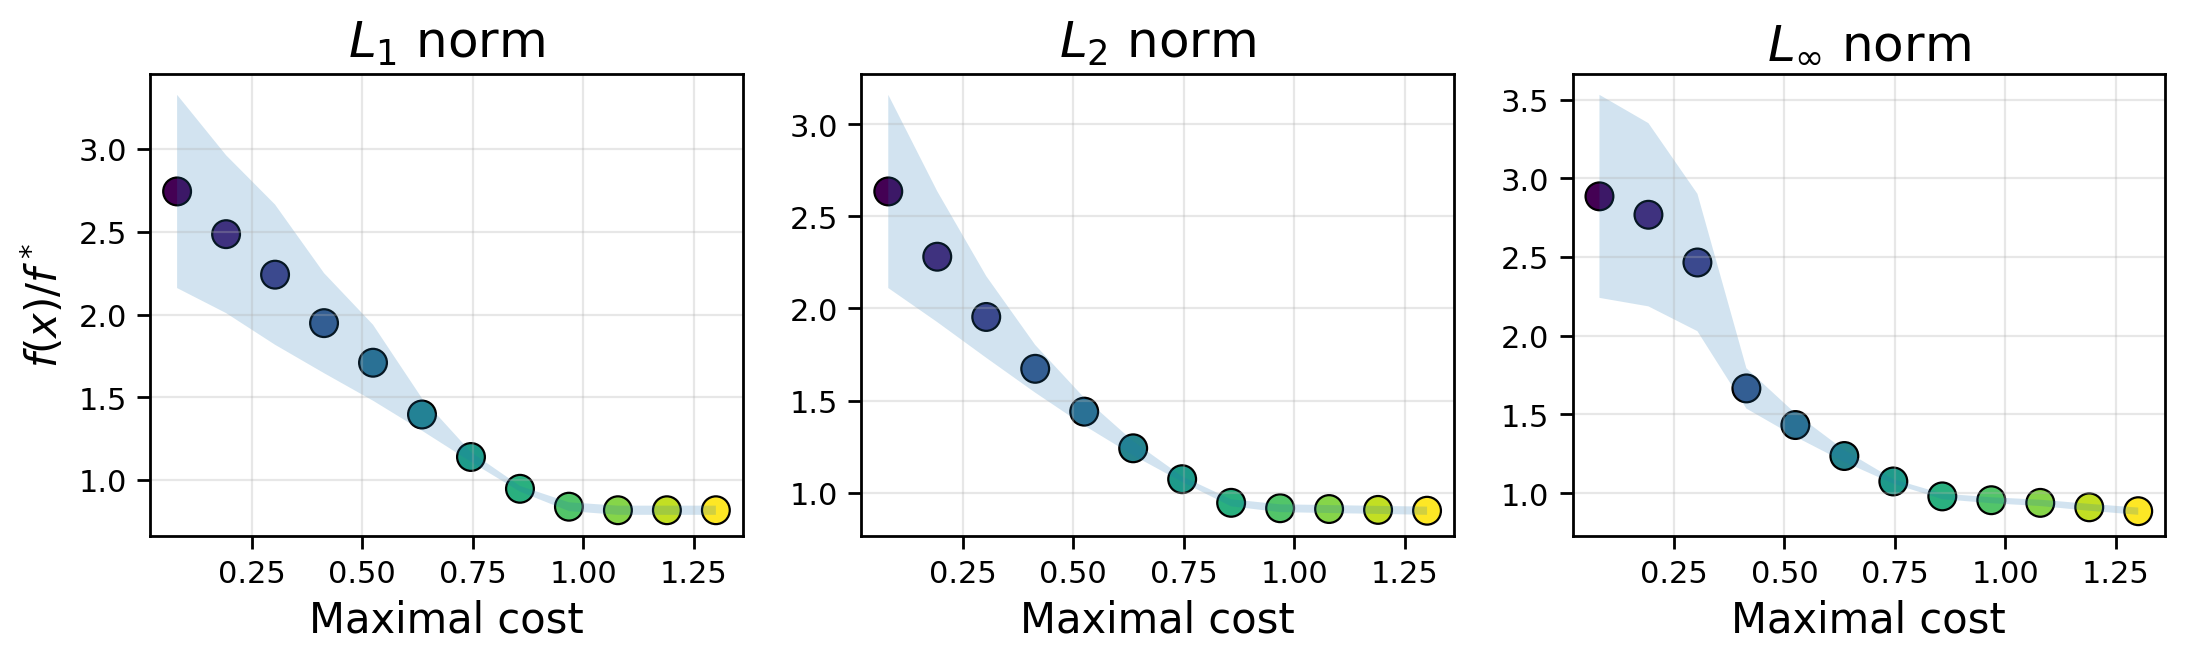
\includegraphics[width=\textwidth]{figures/mcf/relations.png}
            \caption{ Зависимость относительного прироста функции в зависимости от бюджета для разных способов решения задачи MCF.}
\label{fig:mcf:relations}
\end{figure}
    
\begin{figure}
    \centering
    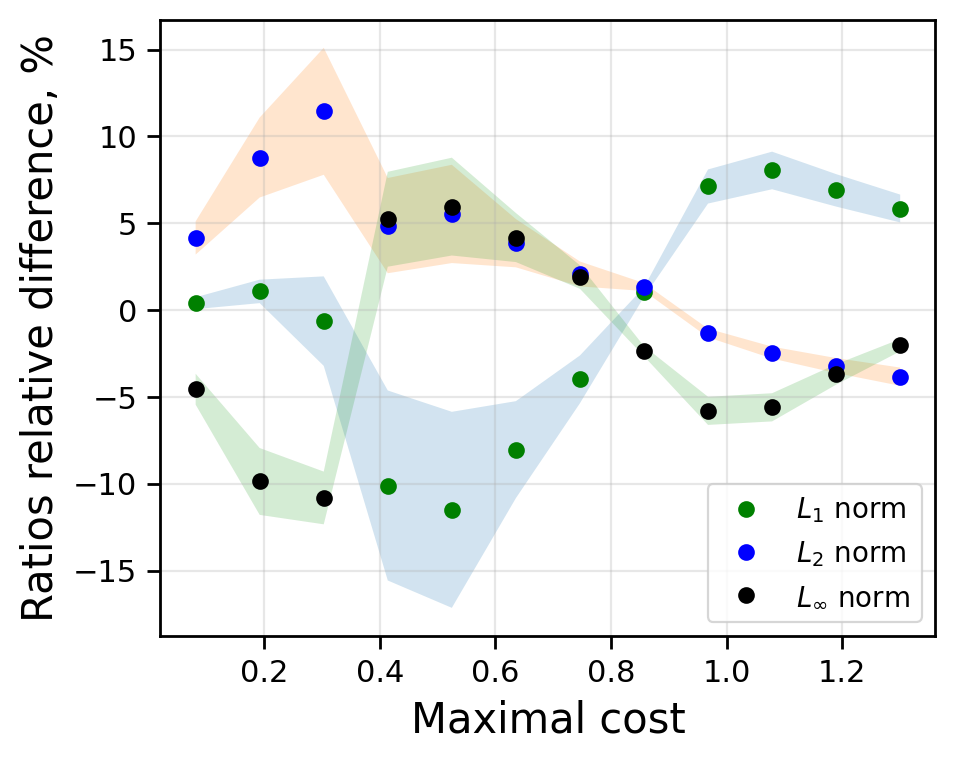
\includegraphics[width=0.5\textwidth]{figures/mcf/relative_difference.png}
    \caption{ Относительная разность качеств приближенного решения со средним качеством решения для задачи MCF.}
    \label{fig:mcf:relative_diff}
\end{figure}

